\chapter{多维随机变量及其分布}
\section{二维随机变量及其分布}
\subsection{二维随机变量}
\dfn{二维随机变量}{
    设随机试验的样本空间为$S$,定义在$S$上的实值单值函数$X = X(\omega)\;Y=Y(\omega)$为两个随机变量.称向量$(X,Y )$为定义在$S$上的\vocab{二维随机变量}
    \begin{center}
        i.e.    $\begin{aligned}
                X:S     & \to\RR    \\
                Y:S     & \to\RR    \\
                (X,Y):S & \to\RR[2]
            \end{aligned}$
    \end{center}
}
类似地,我们可以得到$n$维随机变量的定义.
\subsection{二维随机变量的分布函数}
\dfn{二维随机变量的分布函数}{
    设$(X,Y)$是二维随机变量,对于任意实数$x,y$,定义二元函数
    \begin{equation}
        F(x,y) = \Pr{X\leq x\cap Y\leq y} \defeq \Pr{X\leq x, Y\leq y}
    \end{equation}
    称为二维随机变量$(X,Y)$的\vocab{分布函数},或\vocab{联合分布函数(Joint CDF)}.
}
\begin{figure}[h]
    \centering
    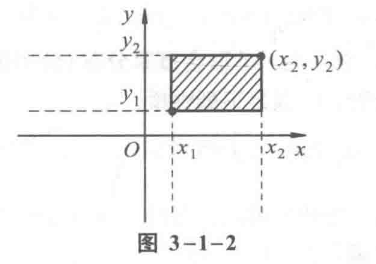
\includegraphics[scale=.6]{jointCDF}
    \caption{CDF}
\end{figure}
将这个向量视作平面内随机点的座标,分布函数就是随机点$(X,Y)$落入矩形域的概率.通过容斥原理计算得到
\begin{equation}
    \Pr{x_1\leq X \leq x_2, y_1\leq Y\leq y_2} = F(x_2,y_2) - F(x_1,y_2) - F(x_2,y_1) + F(x_1,y_1)
\end{equation}
\newpage
\subsubsection{联合CDF的性质}
\leftnote[1cm]{右侧几个等式可通过矩形域的面积来理解.}
\begin{enumerate}
    \item $0\leq F(x,y )\leq 1$
          \begin{enumerate}
              \item 固定$y$,$F(-\infty,y ) = 0$;
              \item 固定$x$,$F(x,-\infty) = 0$;
              \item $\lim_{\substack{x\to +\infty\\y\to +\infty}}F(x,y ) = 1, \lim_{\substack{x\to -\infty\\y\to -\infty}}F(x,y) = 0$
          \end{enumerate}
    \item (\textit{单调性})$F(x,y )$关于$x$和$y$都是单调不减的.
          \begin{enumerate}
              \item 固定$y$,$F(x,y )$关于$x$单调不减;
              \item 固定$x$,$F(x,y )$关于$y$单调不减.
          \end{enumerate}
    \item (\textit{连续性})$F(x,y )$关于$x$和$y$都是右连续的.
\end{enumerate}
若已知$(X,Y)$的分布函数$F(X,Y)$,则可由之导出各个参数(在固定另一个参数的情况下)各自的分布函数:
\begin{align}
    F_X(X) & = \Pr{X\leq x } =\Pr{X\leq x} = \lim_{y\to +\infty}F(x,y), \\
    F_Y(y) & = \Pr{Y\leq y } =\Pr{Y\leq y} = \lim_{x\to +\infty}F(x,y),
\end{align}
如此导出的CDF称为\vocab{边缘分布函数}.
\subsection{二维离散型随机变量及其分布律}
\dfn{联合概率分布律}{
    设$(X,Y)$是二维离散型随机变量,若存在非负函数$p_{ij}$,使得
    \begin{equation}
        \Pr{X=x_i,Y=y_j} = p_{ij},\quad i,j=1,2,\cdots
    \end{equation}
    则称$(X,Y)$为二维离散型随机变量,并称$p_{ij}$为$(X,Y)$的\vocab{联合概率分布律}.
}
显然,$p_{ij}$满足性质:\;\;
\begin{enumerate*}
    \item $p_{ij}\geq 0$;
          \quad\item $\sum_i\sum_j p_{ij} = 1$.
\end{enumerate*}
利用其分布律,易见$(X,Y )$在$D$上的概率为
\begin{equation}
    \Pr{(X,Y)\in D} = \sum_{(x_i,y_j)\in D}p_{ij}
\end{equation}
而其联合CDF为
\begin{equation}
    F(x,y) = \Pr{X\leq x, Y\leq y } = \sum_{x_i\leq x,\,y_j\leq y}p_{ij}
\end{equation}
\subsubsection{边缘分布律}
通过联合概率分布,我们可以得到$X,Y$各自的概率分布:
\leftnote[.5cm]{即行和,列和}
\begin{align}
    p_{i\cdot}  & = \Pr{X=x_i} = \sum_j p_{ij} \\
    p_{\cdot j} & = \Pr{Y=y_j} = \sum_i p_{ij}
\end{align}
这称为$(X,Y)$的\vocab{边缘分布}.
\qs{例1}{设随机整数变量$X=1,2,3,4$,$Y=1\sim X$等可能地取值,试求$(X,Y)$的分布律.}
\sol{
    \begin{align*}
        \mbox{由题意可得}\Pr{X=i,Y=j} & = \Pr{Y=j|X=i}\Pr{X=i}\eqref{eq:mul}                   \\
                                 & = \frac{1}{i }\cdot\frac{1 }{4 }, i =1,2,3,4, j\leq i.
    \end{align*}
    \begin{center}
        \begin{tabular}{|c|c|c|c|c|}
            \hline
            $X,Y$ & $1$    & $2$    & $3$    & $4$    \\ \hline
            $1$   & $1/4$  & $0$    & $0$    & $0$    \\ \hline
            $2$   & $1/8$  & $1/8$  & $0$    & $0$    \\ \hline
            $3$   & $1/12$ & $1/12$ & $1/12$ & $0$    \\ \hline
            $4$   & $1/16$ & $1/16$ & $1/16$ & $1/16$ \\ \hline
        \end{tabular}
    \end{center}
}
\subsection{二维连续型随机变量及其概率密度}
\dfn{二维连续型随机变量}{
    设$(X,Y)$是二维随机变量,$F(X,Y)$为其分布函数,若存在非负可积函数$f(x,y)$ s.t.
    \begin{equation*}
        F(x,y) = \int_{-\infty}^x\int_{-\infty}^y f(u,v)\dd{u}\dd{v}
    \end{equation*}
    则称$(X,Y)$为\vocab{二维连续型随机变量},称$f(x,y)$为其\vocab{概率密度}
}
显然,$f(x,y)$满足性质:\;\;
\begin{enumerate*}
    \item $f(x,y)\geq 0$;
    \item \quad$\int_{-\infty}^{+\infty}\int_{-\infty}^{+\infty}f(x,y)\dd{x}\dd{y} =F(+\infty,+\infty)=1$.
\end{enumerate*}

\textbf{重要性质}\quad 设$D$是$xOy$平面上的区域,$(X,Y )$落入其中的概率为
\begin{equation}
    \Pr{(X,Y)\in D} = \iint_D f(x,y)\dd{x}\dd{y}
\end{equation}
若$f(x,y)$在$(x,y )$处连续,则有
\begin{equation}
    \frac{\partial^2 F(x,y)}{\partial x\partial y} = f(x,y).
\end{equation}
\subsubsection{边缘概率密度}\label{sec:marginPDF}
我们知道此处的$X$和$Y$都是都是连续型随机变量,可得它们的\vocab{边缘密度}为
\begin{align}
    f_X(x)=\int_{-\infty}^{+\infty}f(x,y )\dd y; &  & f_Y(y)=\int_{-\infty}^{+\infty}f(x,y )\dd x;
    \label{eq:3.12}
\end{align}
结合之前的性质,我们可以知道对$F(x,y)$求一个变量的偏导可以得到另一个变量的边缘密度.
\leftnote[2cm]{通常都是分段函数,且一段为$0$\\(\textit{不然很难算})}
\exc{习题3-1-6改}{
    设随机变量$(X,Y )$的概率密度为
    \begin{align*}
        f(x,y) = \begin{cases}
                     k(6-x-y), & 0<x<2, 2<y<4 \\
                     0,        & \mbox{else}
                 \end{cases}
    \end{align*}
    求\begin{enumerate*}
        \item 常数$k$;
        \item \;\;$\Pr{X+Y \leq 4}$;
        \item \;\;$X,Y$的边缘密度.
    \end{enumerate*}
}
\sol{
(1)因为

\begin{align*}
    \int_{-\infty}^{+\infty}\int_{-\infty}^{+\infty}f(x,y)\dd{x}\dd{y} =\begin{cases}
                                                                            \iint_Dk(6-x-y)\dd x\dd y, & x\in D={(x,y)|x\in (0,2) y\in (2,4)} \\
                                                                            0,                         & \mbox{else}
                                                                        \end{cases} =1
\end{align*}
即
\[\iint_Dk(6-x-y )\dd x\dd y = \int_{0}^{2}\int_{2}^{4}k(6-x-y )\dd x\dd y = 1,\mbox{计算可得}k = \frac{1}{8}.\]
\newpage
\noindent (2)由题意,所有符合的$(X,Y)$至少落在直线$x + y = 4$的左侧.由(1)知点只可能落入$D$中,故令\\$G = D\cap \{x+y\leq 4\}$,即下图{\color[HTML]{8e3a16}\textit{棕色区域}}
    \leftnote[1.8cm]{Geogebra画图转TikZ十分好用.}
    \begin{center}
        \usetikzlibrary{arrows}
\definecolor{zzttqq}{rgb}{0.6,0.2,0}
\definecolor{xdxdff}{rgb}{0.49019607843137253,0.49019607843137253,1}
\definecolor{uuuuuu}{rgb}{0.26666666666666666,0.26666666666666666,0.26666666666666666}
\begin{tikzpicture}[line cap=round,line join=round,>=triangle 45,x=1cm,y=1cm,scale=.6,thick]
    \begin{axis}[
            x=1cm,y=1cm,
            axis lines=middle,
            xmin=-1.0430999574123194,
            xmax=4.793645986891604,
            ymin=-0.3419648743673125,
            ymax=4.411066384011339,
            xtick={-1,0,...,4},
            ytick={0,1,...,4},]
        \clip(-1.0430999574123194,-0.3419648743673125) rectangle (4.793645986891604,4.411066384011339);
        \fill[line width=2pt,color=zzttqq,fill=zzttqq,fill opacity=0.10000000149011612] (0,4) -- (0,2) -- (2,2) -- cycle;
        \draw [line width=2pt,domain=-1.0430999574123194:4.793645986891604] plot(\x,{(--4-1*\x)/1});
        \draw [line width=2pt,color=zzttqq] (0,4)-- (0,2);
        \draw [line width=2pt,color=zzttqq] (0,2)-- (2,2);
        \draw [line width=2pt,color=zzttqq] (2,2)-- (0,4);
        \begin{scriptsize}
            \draw[color=black] (0.5,4.184310865488937) node {$eq1$};
            \draw [fill=uuuuuu] (0,4) circle (2pt);
            \draw [fill=xdxdff] (0,2) circle (2.5pt);
            \draw [fill=xdxdff] (2,2) circle (2.5pt);
        \end{scriptsize}
    \end{axis}
\end{tikzpicture}
    \end{center}
    那么,我们有
    \[k\cdot\iint_G6-x-y \dd x\dd y = \Pr{X+Y\leq 4}= \frac{2}{3}\;\;\mbox{即为所求}.\]
    \leftnote[2cm]{相当于固定一个变量,对另一个变量积分}
    (3)根据\ref{sec:marginPDF},可以得到
    \begin{align*}
        f_X(x) & = \begin{cases}
                       {\displaystyle\frac{1}{8}\cdot\int_{2}^{4-x}(6-x-y)\dd y = \frac{1}{8}(6-4x+\frac{1}{2}x^2)}, & 0<x<2       \\
                       0,                                                                                            & \mbox{else}
                   \end{cases}                                          \\
               & \mbox{同理可得}                                                                                                                                              \\
        f_Y(y) & = \begin{cases}
                       {\displaystyle\frac{1}{8}\cdot\int_{0}^{4-y}(6-x-y)\dd x = \mbox{(\dots\;略)}},\hphantom{(4x+\frac{1}{2}x^2)} & 2<y<4       \\
                       0,                                                                                                           & \mbox{else}
                   \end{cases}
    \end{align*}
    }
    \subsection{二维均匀分布}
    \dfn{二维均匀分布}{
        设$G$是平面上的有界区域,其面积为$A$,若二维随机变量$(X,Y )$具有概率密度函数
        \begin{align}
            f(x,y)=\begin{cases}
                       \frac{1}{A}, & (x,y)\in G  \\
                       0,           & \mbox{else}
                   \end{cases}
        \end{align}
        则称$(X,Y )$在$G$上服从二维均匀分布,记为$(X,Y)\sim U(G)$.
    }
    \begin{wrapfigure}[4]{r}{95pt}
        \begin{center}
            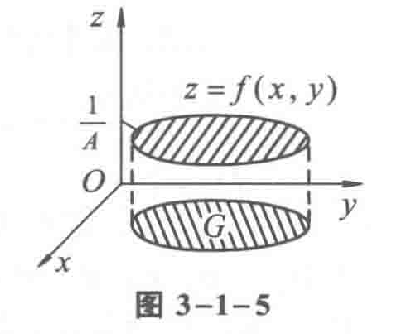
\includegraphics[scale=.5]{2dUniform}
        \end{center}
        \caption{均匀分布}
    \end{wrapfigure}
    若$(X,Y)$在$G$上服从均匀分布,则其概率密度函数反映在几何上为定义在$xOy$平面内区域$G$上的空间的一块平面.
    考虑向平面$G$上投掷一质点,若点落在区域$B\subset G$内的概率与$B$的面积成正比且与$B$的位置无关,则称$G$为均匀分布的区域,
    座标$(X,Y)$在$G$上服从均匀分布.
\leftnote[2.5cm]{\color{red}对于\textbf{矩形域}$G$该公式成立,其他形状则不一定.}
\cor{}{
    均匀分布$(X,Y)$的两个边缘分布仍为均匀分布且分别为
    \begin{align}
        \begin{split}
            f_X(x) & = \begin{cases}
                \frac{1}{b-a}, & a<x<b       \\
                0,             & \mbox{else}
            \end{cases} \\
            f_Y(y) & = \begin{cases}
                \frac{1}{d-c}, & c<y<d       \\
                0,             & \mbox{else}
            \end{cases}
        \end{split}
    \end{align}
}

\qs{例5}{
    设$(X,Y)$服从\textit{单位圆域}上的均匀分布,求对应的两个边缘分布.
}
\newpage
\sol{
    由题意得,其PDF为
    \begin{align*}
        f(x,y) & = \begin{cases}
                       \frac{1}{\pi}, & x^2+y^2\leq 1 \\
                       0,             & \mbox{else}
                   \end{cases}
    \end{align*}
    根据\eqref{eq:3.12},只需考虑点在圆域内的情况,易得
    \begin{align*}
        f_X(x)     & = \int_{-\sqrt{1-x^2}}^{\sqrt{1-x^2}}\frac{1}{\pi}\dd y = \frac{2}{\pi}\sqrt{1-x^2}. \\
        \tf f_X(x) & = \begin{cases}
                           \frac{2}{\pi}\sqrt{1-x^2}, & -1\leq x\leq 1 \\
                           0,                         & \mbox{else}
                       \end{cases}
    \end{align*}
    因为$x^2 + y^2 \leq 1$是\textit{轮换式},将$x$换成$y$即可得到$f_Y(y)$.
}